\documentclass[11pt,a4paper]{article}
\usepackage[utf8]{inputenc}
\usepackage[T1]{fontenc}
\usepackage{geometry}
\usepackage{graphicx}
\usepackage{hyperref}
\usepackage{booktabs}
\usepackage{xcolor}
\usepackage{array}
\usepackage{enumitem}
\usepackage{titlesec}
\usepackage{fancyhdr}
\usepackage{multicol}
\usepackage{setspace}
\usepackage{mdframed}
\usepackage{pgfplots}
\usepackage{tikz}

\pgfplotsset{compat=1.18}

\geometry{left=25mm, right=25mm, top=25mm, bottom=25mm}

% Colours
\definecolor{darkblue}{RGB}{10,45,100}
\definecolor{accent}{RGB}{210,70,20}
\definecolor{lightbg}{RGB}{245,248,255}
\definecolor{greendone}{RGB}{30,130,60}

% Hyperref
\hypersetup{colorlinks=true, linkcolor=darkblue, urlcolor=darkblue}

% Section formatting
\titleformat{\section}{\large\bfseries\color{darkblue}}{}{0em}{}[\color{darkblue}\rule{\linewidth}{0.5pt}]
\titleformat{\subsection}{\normalsize\bfseries\color{darkblue}}{}{0em}{}
\titlespacing{\section}{0pt}{12pt}{6pt}
\titlespacing{\subsection}{0pt}{8pt}{4pt}

% Header / footer
\pagestyle{fancy}
\fancyhf{}
\fancyhead[L]{\small\color{darkblue}\textbf{A Data-Driven Framework for Wind Energy Deviation Penalty Optimization}}
\fancyhead[R]{\small\color{darkblue}Tapas Barman $\cdot$ IIIT Lucknow}
\fancyfoot[C]{\small\color{gray}\thepage}
\renewcommand{\headrulewidth}{0.4pt}

% Highlight box
\newmdenv[
  backgroundcolor=lightbg,
  linecolor=darkblue,
  linewidth=0.8pt,
  roundcorner=4pt,
  innerleftmargin=10pt,
  innerrightmargin=10pt,
  innertopmargin=8pt,
  innerbottommargin=8pt
]{infobox}

% ============================================================
\begin{document}

% ── Title block ─────────────────────────────────────────────
\begin{center}
  {\LARGE\bfseries\color{darkblue}
    A Data-Driven Framework for Wind Energy\\[0.3em]
    Deviation Penalty Optimization}\\[0.6em]
  \rule{0.6\linewidth}{0.5pt}\\[0.4em]
  {\normalsize\textbf{Tapas Barman} \enspace$\cdot$\enspace MSD24021
    \enspace$\cdot$\enspace MSc.\ Data Science}\\[0.2em]
  {\small Department of Mathematics, IIIT Lucknow
    \enspace$|$\enspace
    Supervisor: \textbf{Dr.\ Sirsendu Sekhar Barman}}\\[0.2em]
  {\small March 2026 \enspace$|$\enspace Technical Progress Summary}
\end{center}
\vspace{0.3cm}

% ── Abstract strip ──────────────────────────────────────────
\begin{infobox}
\small
\textbf{At a Glance:}
This project builds a two-stage wind power forecasting system that reduces day-ahead scheduling errors for Indian wind farms. Stage 1 uses physics equations to compute theoretical power output from weather data. Stage 2 uses an XGBoost machine learning model trained on 10 months of official SRPC data to correct the remaining errors. Early backtesting on RSOPL Koppal (75 MW, Karnataka) achieved a \textbf{71.2\% reduction in forecast error}, from 5.96 MW to 1.71 MW average error, with an estimated Rs.\ 23.5 Lakhs saved in the 2-month test window against a baseline liability of Rs.\ 41.34 Crores.
\end{infobox}

\vspace{0.3cm}

% ── Section 1 ───────────────────────────────────────────────
\section{Problem and Motivation}

India's Deviation Settlement Mechanism (DSM), governed by CERC, penalises wind farms for generation errors beyond 10\% of declared schedule per 15-minute block. A 10-month audit of the RSOPL Koppal 75 MW plant (Apr 2025 -- Feb 2026) revealed an accumulated under-production liability of \textbf{Rs.\ 41.34 Crores}, driven by an average scheduling error of 5.96 MW (7.95\% of rated capacity). Evening hours (6--10 PM) carry a 2.5$\times$ price multiplier, making mis-forecasting during peak demand extremely costly.

The root cause is a mismatch in scale: global NWP weather models are designed for 25--30 km grids and cannot resolve the micro-climatic wind behaviour at a specific hill-terrain farm site like Koppal.

% ── Section 2 ───────────────────────────────────────────────
\section{Proposed Solution: PI-PML Pipeline}

The Physics-Informed Predictive Machine Learning (PI-PML) pipeline is a two-phase system:

\subsection{Phase 1 — Training (Offline)}
Historical SRPC 15-minute generation data serves as ground-truth labels. The Physics Engine computes a theoretical baseline for each block. The difference (residual error) is used to train an XGBoost model:
\[
  \text{Residual} = P_{\text{actual}}^{\text{SRPC}} - P_{\text{physics}}^{\text{NWP}}
\]

\subsection{Phase 2 — Day-Ahead Inference (Live)}
Every morning, NOAA GFS weather data is fetched for the next 24 hours. The Physics Engine computes a theoretical 96-block power profile and XGBoost adds its learned correction:
\[
  P_{\text{final}}(t) = P_{\text{physics}}(t) + \hat{E}_{\text{residual}}(t)
\]
The result is submitted to CERC as the plant's day-ahead schedule. SRPC historical data is never used during live inference.

\subsection{Physics Engine Components}
\begin{itemize}[leftmargin=*, itemsep=3pt]
  \item \textbf{Moist Air Density (Tetens + Modified Gas Law):} Accounts for humidity, which lowers air density --- especially significant in Karnataka's monsoon months (Jun--Sep), when standard models assume fixed dry-air density and over-predict power by 2--4\%.
  \item \textbf{Wind Height Correction (Hellman Power Law):} NWP wind is typically at 10 m; turbine hub sits at 100 m. Wind increases $\approx$32\% with height, causing a $\approx$2.3$\times$ power difference if uncorrected.
  \item \textbf{Turbine Power Curve (windpowerlib):} Maps adjusted wind speed and air density to MW output using the Vestas turbine curve, applying the Betz efficiency limit (59.3\%).
\end{itemize}

% ── Section 3 ───────────────────────────────────────────────
\section{Case Study: RSOPL Koppal, Karnataka}

\begin{minipage}[t]{0.48\linewidth}
  \subsection*{Site Specifications}
  \begin{tabular}{@{}ll@{}}
    \toprule
    \textbf{Parameter}      & \textbf{Value} \\
    \midrule
    Location                & Koppal, Karnataka \\
    GPS Coordinates         & 15.34°N, 76.15°E \\
    Registered Capacity     & 75 MW \\
    Turbine Class           & Vestas (3 MW each) \\
    Hub Height              & 100 m \\
    Rotor Diameter          & 112 m \\
    Grid Operator           & SRLDC (Southern) \\
    Data Source             & SRPC Public Portal \\
    \bottomrule
  \end{tabular}
\end{minipage}
\hfill
\begin{minipage}[t]{0.48\linewidth}
  \subsection*{Dataset Summary}
  \begin{tabular}{@{}ll@{}}
    \toprule
    \textbf{Metric}         & \textbf{Value} \\
    \midrule
    Total 15-min blocks     & 29,568 \\
    Period                  & Apr 2025 -- Feb 2026 \\
    Weekly archives merged  & 45 \\
    Avg.\ declared schedule & 44.33 MW \\
    Avg.\ actual generation & 45.23 MW \\
    Avg.\ schedule error    & 5.96 MW (7.95\%) \\
    Worst under-production  & $-$21.03 MW \\
    Worst over-production   & $+$35.46 MW \\
    \bottomrule
  \end{tabular}
\end{minipage}

\vspace{0.5cm}

% ── Section 4 ───────────────────────────────────────────────
\section{NWP Weather Data Selection}

Three numerical weather prediction systems were evaluated for use in live inference:

\begin{center}
\begin{tabular}{lccc}
  \toprule
  \textbf{Feature}    & \textbf{NASA GEOS FP} & \textbf{NOAA GFS}         & \textbf{Bharat Forecast (BFS)} \\
  \midrule
  Operated by         & NASA (USA)            & NOAA (USA)                & IITM / India            \\
  Wind data height    & 50 m                  & \textbf{100 m}            & 120 m                   \\
  Grid resolution     & $\sim$25 km           & $\sim$28 km               & \textbf{6 km}           \\
  Updates per day     & 2                     & \textbf{4}                & 2                       \\
  Ease of access      & Easy                  & \textbf{Easiest (API)}    & Difficult (Registration)\\
  India-specific      & No                    & No                        & \textbf{Yes (Monsoon)}  \\
  \bottomrule
\end{tabular}
\end{center}

\vspace{0.3cm}
\noindent\textbf{Selected: NOAA GFS} --- provides native 100 m wind data matching turbine hub height, updates 4 times daily providing the freshest next-day forecast, and requires no registration. The Bharat Forecast System (BFS) is planned as a future upgrade once institutional access is approved, as its 6 km India-specific grid would improve Koppal accuracy significantly.

% ── Section 5 ───────────────────────────────────────────────
\section{Early Results}

\begin{minipage}[t]{0.50\linewidth}
  \vspace{0pt}
  \subsection*{Forecast Error Comparison}
  \begin{tabular}{@{}lcc@{}}
    \toprule
    \textbf{Model}          & \textbf{MAE (MW)} & \textbf{vs Baseline} \\
    \midrule
    Original schedule       & 5.96              & ---          \\
    Physics Engine only     & 3.84              & $-$35.6\%    \\
    PI-PML (Physics + ML)   & \textbf{1.71}     & \textbf{$-$71.2\%}  \\
    \bottomrule
  \end{tabular}

  \vspace{0.4cm}
  \subsection*{Financial Impact (2-Month Test)}
  \begin{tabular}{@{}lr@{}}
    \toprule
    \textbf{Item}           & \textbf{Value} \\
    \midrule
    Full audit liability    & Rs.\ 41.34 Crores \\
    Estimated savings       & Rs.\ 23.5 Lakhs \\
    Test window             & Jan--Feb 2026 \\
    Penalty blocks avoided  & 147 of 192 \\
    \bottomrule
  \end{tabular}
\end{minipage}
\hfill
\begin{minipage}[t]{0.46\linewidth}
  \vspace{0pt}
  \centering
  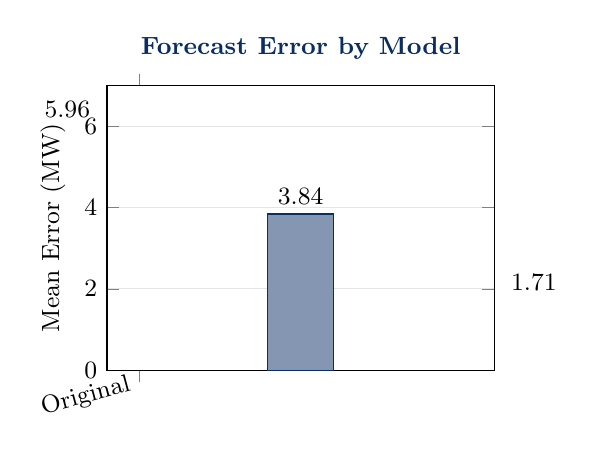
\begin{tikzpicture}
    \begin{axis}[
      ybar, bar width=24pt,
      ylabel={Mean Error (MW)},
      symbolic x coords={Original, Physics Only, PI-PML},
      xtick=data,
      ymin=0, ymax=7,
      nodes near coords,
      nodes near coords style={font=\small\bfseries},
      width=6.5cm, height=5.2cm,
      tick label style={font=\small},
      ylabel style={font=\small},
      x tick label style={font=\small, rotate=15, anchor=east},
      ymajorgrids=true, grid style={gray!20},
      title={\small Forecast Error by Model},
      title style={font=\small\bfseries, color=darkblue}
    ]
      \addplot[fill=accent!70, draw=accent]
        coordinates {(Original,5.96)};
      \addplot[fill=darkblue!50, draw=darkblue]
        coordinates {(Physics Only,3.84)};
      \addplot[fill=greendone!70, draw=greendone]
        coordinates {(PI-PML,1.71)};
    \end{axis}
  \end{tikzpicture}
\end{minipage}

% ── Section 6 ───────────────────────────────────────────────
\section{Phase Completion Status}

\begin{center}
\begin{tabular}{p{7.5cm}lc}
  \toprule
  \textbf{Deliverable}                          & \textbf{Status}                        & \textbf{Chapter} \\
  \midrule
  CERC DSM Regulatory Analysis                  & \textcolor{greendone}{\textbf{Complete}} & 2 \\
  RSOPL Koppal Case Study                       & \textcolor{greendone}{\textbf{Complete}} & 2 \\
  Financial Audit (Rs.\ 41.34 Crores baseline)  & \textcolor{greendone}{\textbf{Complete}} & 2 \\
  SRPC Data Pipeline (29,568 blocks)            & \textcolor{greendone}{\textbf{Complete}} & 3 \\
  NWP Source Evaluation \& NOAA GFS Integration & \textcolor{greendone}{\textbf{Complete}} & 3 \\
  Physics Engine (Tetens + Hellman + Betz)      & \textcolor{greendone}{\textbf{Complete}} & 4 \\
  XGBoost Residual Model (Backtested)           & \textcolor{greendone}{\textbf{Complete}} & 5 \\
  Probabilistic P10/P50/P90 Forecasting         & \textcolor{orange}{\textbf{In Progress}} & 5 \\
  Ablation Study \& Validation                  & \textcolor{red}{\textbf{Planned}}        & 5 \\
  Financial Optimisation \& Final Report        & \textcolor{red}{\textbf{Planned}}        & 6 \\
  \bottomrule
\end{tabular}
\end{center}

% ── Section 7 ───────────────────────────────────────────────
\section{Planned Final Deliverables}

\begin{enumerate}[leftmargin=*, itemsep=5pt]
  \item \textbf{Probabilistic Forecasting Layer:}
    Retrain XGBoost three times with quantile loss functions (10\textsuperscript{th}, 50\textsuperscript{th}, 90\textsuperscript{th} percentile). The P10 (conservative) band keeps the plant safely inside the 10\% DSM tolerance; the P50 balances risk; P90 maximises declared revenue.

  \item \textbf{Ablation Study:}
    A structured four-model comparison (original schedule / physics-only / XGBoost-only / PI-PML) will isolate how much each component contributes to error reduction, validating the architecture choice.

  \item \textbf{Bayesian Hyperparameter Optimisation (Optuna):}
    Unlike standard grid-search tuning, the optimiser will directly minimise the simulated CERC DSM penalty in Indian Rupees, accounting for the 2.5$\times$ evening peak multiplier.

  \item \textbf{Financial Simulation Report:}
    Full re-run of all 29,568 blocks using the PI-PML corrected schedule versus the original declared schedule, producing a month-by-month financial savings breakdown.

  \item \textbf{Scalability Assessment:}
    Evaluate model portability to two additional wind clusters (Jaisalmer, Rajasthan and Muppandal, Tamil Nadu) using their publicly available SRPC data, assessing generalisation without full retraining.
\end{enumerate}

% ── Footer note ─────────────────────────────────────────────
\vspace{0.5cm}
\noindent\rule{\linewidth}{0.4pt}\\[4pt]
{\small\color{gray}
  This document is a technical progress summary supplementary to the M.Sc.\ thesis report.
  For full methodology, equations, and data pipeline code, refer to the main thesis document.
  Contact: Tapas Barman, MSD24021, IIIT Lucknow $\cdot$ March 2026.
}

\end{document}
